\documentclass[9pt]{beamer}
% \special{dvipdfmx:config z 0}	% 取消PDF压缩
\AddToHook{package/xeCJK/after}{\defaultCJKfontfeatures{}}
\usepackage{ctex}
\usepackage{amssymb}
\usepackage{amsmath}
\usepackage{graphicx}
\usepackage{multirow}
\usepackage{natbib}
\usepackage{subcaption}
\usepackage{tabulary}
\usepackage{SDU}

\author{刘纯彰}
\title{物理化学辅导课}
\institute{Qingdao Institute for Theoretical and Computational Sciences\\ Shandong University}
\date{\today}

% new command created
%% for mathematical application
\newcommand\A{{\rm A}}
\newcommand\B{{\rm B}}
\newcommand\C{{\rm C}}
\newcommand\amb{{\rm amb}}
\newcommand*{\dif}{\mathop{}\!\mathrm{d}}
\newcommand\cc{{\rm c}}
\newcommand\bb{{\rm b}}
\newcommand\f{{\rm f}}
\newcommand\K{{\rm K}}
\newcommand\m{{\rm m}}
\newcommand\rr{{\rm r}}
\newcommand{\s}{{\rm s}}
%% for article format
\newcommand\Figref[1]{Fig \ref{#1}}
\newcommand\Tableref[1]{Table \ref{#1}}
\newcommand\Eqref[1]{Eq.\,\eqref{#1}}
\newcommand\Secref[1]{Sec.\,\thesec\stepcounter{sec}}
\def\CC{{C\nolinebreak[4]\hspace{-.05em}\raisebox{.4ex}{\tiny\bf ++}}}

% some caption setup
%\captionsetup[figure]{labelfont={bf},labelsep=period,name={FIG }}
%\captionsetup[table]{labelfont={bf},labelsep=period,name={TABLE }}

\setcitestyle{super, square}
\usefonttheme[onlymath]{serif}
%\setbeamerfont*{size}{\small}
\bibliographystyle{unsrt}

% my counter
\newcounter{mycnt}
\setcounter{mycnt}{0}

\begin{document}

	\begin{frame}
    	\titlepage
    	\begin{figure}[htb]
           	 
\includegraphics[width=0.15\linewidth]{./pictures/SDUlogo.jpg}
		\end{figure}
	\end{frame}

	\begin{frame}
    	\tableofcontents[sectionstyle=show,subsectionstyle=show/shaded/hide]
	\end{frame}

	\section{课程简介及导论}
	
	\subsection{物理化学的学科性质和原则}

	\begin{frame}
	
	如何学习物理化学?
	
	\hspace*{\fill}	
	
	首先意识到物理化学的学科性质:它是一门{\color{red}公理化}的{\color{red}唯象学科}。特点为
	
	\begin{enumerate}
	
	\item {\color{red}推导前提}和{\color{red}适用对象}最重要。
	
	\item 定律、原理和物理对应比公式重要。
	
	\item 计算是最后一步。
	
	\end{enumerate}
	
	\hspace*{\fill}
	
	物理化学中处理问题要规范,体现在三个方面:
	\begin{enumerate}
	

	\item 首先明确{\color{red}物理对象}与{\color{red}变化情况}。
	
	\item {\color{red}有效数字}处理要规范,如加法可能损失有效数字但乘法不损失。	
	
	\item {\color{red}运算时携带量纲},尽量避免换算导致的错误。	
	
	\end{enumerate}
	
	\end{frame}

	\subsection{辅导课的课程安排}
	
	\begin{frame}
	
	本辅导课的课程安排如下:	
	\begin{enumerate}
	
	\item 第一章、第二章、第三章
	
		第一章介绍了最常见也是最简单的物质模型——{\color{red}(理想)气体}。
		
		第二章、第三章共同描述了单一组分体系下的{\color{red}热力学定律}和{\color{red}诸多过程}。
	
	\item 第四章、第五章
	
		第四章引入了{\color{red}化学势}以描述多组分系统的热力学性质。在此过程中,引入了两个新的模型,{\color{red}理想液态混合物}和{\color{red}理想稀溶液}。
		
		{\color{blue}从第五章起,其余章节更多的是不同化学体系的原理应用而非原理介绍。}
		
		第五章以{\color{red}化学反应体系}为研究对象,研究其热力学平衡限度。
	
	\item 第六章、第七章
	
		第六章主要以二组分非电解质的理想稀溶液系统为例,用相图来说明{\color{red}物理变化}中的相平衡。
		
		第七章以{\color{red}电解质溶液}为研究对象,介绍了其电导性、{\color{red}热力学}及电极极化现象。
	
	\item 第十章、第十一章和第十二章
	
		第十章以界面为研究对象,研究以表面张力为核心的界面现象。
		
		{\color{blue}从第十一章起,研究内容不再是经典的平衡态热力学。}
		
		第十一章讲述{\color{red}化学动力学},从{\color{red}微观层面}解析{\color{red}具体}的化学反应。
		
		第十二章讲述{\color{red}胶体}这一非热力学稳定体系的各种特殊性质。	
	
	\end{enumerate}
	
	\end{frame}
	
	\section{第一部分}
	
	\subsection{第一章}
	
	\begin{frame}
	
	第一章的主要原理:
	
	\begin{itemize}
	
	\item 理想气体的概念及两个特征
	
	\item 理想气体状态方程:
	\[
		pV = n R T = \frac{m}{M} R T
	\]
	摩尔气体常数$R \approx 8.314\, {\rm J\cdot mol^{-1} \cdot K^{-1}}$
	
	\item Dalton分压定律:$p_\B = x_\B p$	
	
	\item 临界参数:临界温度$T_c$和临界压力$p_c$的概念
	
	\item van der Waals方程:
	\[
		\left( p + \frac{a}{V^2_{\rm m}} \right) ( V_{\rm m} - b ) = RT, \quad V_{\rm m} \equiv \frac{n}{V}
	\]
	
	\item 压缩因子$Z$:
	\[
		Z \equiv \frac{pV}{nRT} = \frac{pV_{\rm m}}{RT} = \frac{V_{\rm m}({\rm real \, gas})}{V_{\rm m}({\rm ideal \, gas})} = f( p_{\rm r}, T_{\rm r} ).
	\]
	$T_{\rm r}$和$p_{\rm r}$为对比温度(即热力学温度与临界热力学温度的比)和对比压力(即压力和临界压力的比)
	\end{itemize}
	
	\end{frame}
	
	\subsection{第二章}
	\begin{frame}
	
	第二章的主要原理:
	
	\begin{itemize}
	
	\item 系统和环境的概念,系统的分类
	
	\item 状态函数的概念,广度性质和强度性质的概念,平衡态的概念
	
	\item 过程函数的概念,体积功和热的概念
	
	\item 热力学第一定律:对仅有体积功的封闭系统,
	\[
		\dif U = \delta W + \delta Q = -p_{\amb} \dif V + Q 
	\]
	
	\item 恒容过程:$\delta Q_V = \dif U$
	
	\item 恒压过程:$\delta Q_p = \dif H$, 此处引入焓$H\equiv U+pV$.
	
	\item Hess定律验证了内能和焓的确是状态函数
	
	\item 摩尔热容的分类
	
		\begin{enumerate}
	
		\item 摩尔定容热容$C_{V,\m}=(\frac{Q_V}{\dif T})_V$,$\dif U = n C_{V,\m} \dif T$
		
		\item 摩尔定压热容$C_{p,\m}=(\frac{Q_p}{\dif T})_p$,$\dif H = n C_{p,\m} \dif T$
		
		\item 理想气体的$C_{p,\m}$与$C_{V,\m}$的关系:$C_{p,\m}-C_{V,\m}=R$
	
		\end{enumerate}
	
	\item 热效应的计算
		\begin{enumerate}
	
		\item 封闭系统不做非体积功的等容过程:$Q_V=\Delta U$
		
		\item 封闭系统不做非体积功的等压过程:$Q_p=\Delta H$
		
		\item 等压热效应和等容热效应之间的关系:$Q_p-Q_V = \Delta n RT$
	
		\end{enumerate}
	
	\end{itemize}
	
	\end{frame}

	\begin{frame}
	
	\begin{itemize}
	
	\item 相、相变、摩尔相变焓的概念
	
	\item 反应进度$\dif \xi$的概念,和化学方程式的关系
	
	\item 标准态、标准摩尔生成焓$\Delta_\f H^{\,\ominus}_\m$的概念
	
	\item 标准摩尔燃烧焓$\Delta_\cc H^{\,\ominus}_\m$的概念
	
	\item 标准摩尔反应焓$\Delta_\rr H^{\,\ominus}_\m$的概念和计算
		\begin{enumerate}
	
		\item $\Delta_\rr H^{\,\ominus}_\m = \sum_\B \nu_\B \Delta_\f H^{\,\ominus}_\m(\B)$
		
		\item $\Delta_\rr H^{\,\ominus}_\m = - \sum_\B \nu_\B \Delta_\cc H^{\,\ominus}_\m(\B)$
	
		\end{enumerate}
	
	\item Kirchhoff公式的前提、适用范围
	\[
		\Delta_\rr H^{\,\ominus}_\m(T) = \Delta_\rr H^{\,\ominus}_\m( 298.15\K ) + \int_{298.15\K}^T \Delta_\rr C_{p,\m} \dif T
	\]
	
	\item 状态函数法构造
	
	\item 可逆过程的概念,理想气体的绝热可逆体积功$W_{a,r} = nC_{V,\m}(T_2-T_1)$	
	
	\item 节流膨胀的概念、物理特征和应用
	
	\end{itemize}		
	
	\end{frame}

	\subsection{第三章}
	\begin{frame}
	
	第三章的主要原理:
	\begin{enumerate}
	
	\item 自发过程和非自发过程的概念
	
	\item 热机效率$\eta$和冷冻系数$\beta$
	\[
		\eta = \frac{-W}{Q_1}, \quad \beta = \frac{Q^\prime_1}{W}
	\]
	
	\item 热力学第二定律的两种表述:Clausius表述和Kelvin表述。
	
	\item Carnot循环的构造,推导热机的最大效率$\eta_{\rm max}$和最大冷冻系数$\beta_{\rm max}$
	
	\[
		\eta_{\rm max} = \frac{T_{\rm h} - T_{\rm c}}{T_{\rm h}}, \quad \beta_{\rm max} = \frac{T_1}{T_2-T_1}
	\]
	
	\item 熵的定义$\dif S = \frac{\delta Q_\rr}{T}$,Clausius不等式、熵增原理的适用对象和内容
	
	\item 熵变的计算思路,核心公式是
	\[
		\dif S = \frac{\delta Q_\rr}{T} = \frac{\dif U + p \dif V}{T} = \frac{\dif H - V \dif p}{T},
	\]
	在恒容情况联立
	\[
		\dif U = n C_{V,\m} \dif T,
	\]
	而在恒压情况联立
	\[
		\dif H = n C_{p,\m} \dif T
	\]
	
	\end{enumerate}
	
	\end{frame}
	
	\begin{frame}
	
	\begin{itemize}
	
	\item 相变过程的熵变计算
		\begin{enumerate}
	
		\item 可逆相变的概念,其直接适用熵的定义式计算
		\[
			\Delta^\beta_\alpha S = \frac{ n \Delta^\beta_\alpha H_\m}{T}.
		\]
	
		\item 不可逆相变的概念,用状态函数法构造热力学循环计算
	
	\end{enumerate}
	
	\item 稳定环境的熵变计算
		\[
			\Delta S_\amb = \frac{ -Q_{\rm sys} }{T_\amb}
		\]
	
	\item 热力学第三定律如何规定了熵的起点
	
	\item 标准摩尔熵$S^{\,\ominus}_\m(T)$,标准摩尔反应熵$\Delta_\rr S^{\,\ominus}_\m = \sum_\B v_\B $
	
	\item Helmholtz函数$A\equiv U-TS$,物理意义及其判据$\dif A_{T,V} \leq 0$
	
	\item Gibbs函数$G\equiv H-TS$,物理意义及其判据$\dif G_{T,p} \leq 0$
	
	\item 热力学基本方程
	\begin{align*}
		\dif U &= T \dif S - p \dif V , \\
		\dif H &= T \dif S + V \dif p , \\
		\dif A &= - S \dif T - p \dif V , \\
		\dif G &= - S \dif T + V \dif p
	\end{align*}		
	
	\end{itemize}		
	
	\end{frame}
	
	\begin{frame}
	
	\begin{itemize}
	
	\item Clapeyron方程适用情形及形式
	\[
		\frac{\dif T}{\dif p} = \frac{ T \Delta^\beta_\alpha V_\m }{ \Delta^\beta_\alpha H_\m }
	\]	
	
	\item Clausius-Clapeyron方程近似条件及形式
	\[
		\frac{\dif p}{\dif T} = \frac{ \Delta^{\rm g}_{\rm l} H_\m }{ T \Delta^{\rm g}_{\rm l} V_\m } = \frac{ \Delta^{\rm g}_{\rm l} H_\m }{ R T^2 }p
	\]
	
	\end{itemize}	
	
	\end{frame}
	
%	\subsection{第一次课后作业情况}
%	\begin{frame}
%	
%	本次课程课堂作业(基础):2.17和3.19	\\
%	\hspace*{\fill}					\\
%	本次课程课后作业(可选):3.35		\\
%	\hspace*{\fill}					\\
%	完成情况:个人记录收到作业13份。
%	规范性普遍做得很有待加强。主要问题包括但不限于
%	\begin{itemize}
%	
%	\item 不写解,仅有3位同学写解
%	
%	\item 缺失对题干中条件的论述
%	
%	\item 没有绘制状态变化示意图,仅有2位同学绘制
%	
%	\item 运算过程中丢失量纲
%	
%	\item 有效数字取舍问题
%	
%	\end{itemize}
%	
%	\hspace*{\fill}					\\	
%	{\color{red}如果觉得我讲课内容无趣,或者无心在此学习但报名了又不能不来,我对于签到后安静离场不打扰课程和其他同学的同学没有任何意见。我个人对于约束同学们的时间和位置没有任何兴趣,签到也不是我事先规定的。}
%	
%	\end{frame}
	
	\section{第二部分}	
	
	\subsection{第四章}
	\begin{frame}
	
	第四章的主要原理:
	\begin{itemize}
	
	\item 系统中,某组分$\B$的状态函数$X$的偏摩尔量的概念,即
	\[
		X_\B \equiv \left( \frac{ \partial X }{ \partial n_\B } \right)_{T,p,n_{\C\neq \B}}
	\]	
	偏摩尔量的物理意义,和摩尔量的联系
	\item Gibbs-Duhem公式及其物理意义(以二组分系统为例)
	
	\item 偏摩尔量之间的两个最重要的函数关系
	\begin{align*}
	\left( \frac{ \partial G_\B }{ \partial p } \right)_T &= V_\B,\\
	\left( \frac{ \partial G_\B }{ \partial T } \right)_p &= -S_\B
	\end{align*}
	
	\item 系统中,某组分$\B$化学势$\mu_\B$的概念
	\[
		\mu_\B \equiv \left( \frac{ \partial G }{ \partial n_\B } \right)_{T,p,n_{\C\neq \B}}
	\]
	
	\item 单相多组分系统的热力学基本方程
	\[
		\dif G = - S \dif T + V \dif p + \sum_\B \mu_\B \dif n_\B
	\]
	
	\end{itemize}
	
	\end{frame}
	
	\begin{frame}
	
	\begin{itemize}
	
	\item 化学势的物理意义及化学平衡表达式
	\[
		\sum_\B \mu_\B \dif n_\B = 0 
	\]
	
	\item 视为理想气体的气体组分的化学势,真实气体的标准态的概念
	\[
		\mu^*({\rm pg}) = \mu^{\,\ominus}({\rm g}) + RT \ln{\frac{p}{p^{\,\ominus}}}
	\]
	
	\item 逸度因子$\varphi_\B$的概念及其物理意义
	
	\item 溶液组成的多种常见表示法,除了摩尔分数$x_\B$外,还有
		\begin{enumerate}
		
		\item 质量摩尔浓度$b_\B$
		\[
			b_\B \equiv \frac{ n_\B }{ m_\A }
		\]
		
		\item 物质的量浓度
		\[
			c_\B \equiv \frac{ n_\B }{ V_\A }
		\]
		\end{enumerate}
	
	\item Raoult定律的适用条件及形式,微观解释
	\[
		p_\A = p^*_\A x_\A
	\]
	
	\item Henry定律的适用条件及形式,微观解释
	\[
		p_\B = k_{x,\B} x_\B = k_{b,\B} b_\B = k_{c,\B} c_\B
	\]
	
	\end{itemize}		
	
	\end{frame}
	
	\begin{frame}
	
	\begin{itemize}
	
	\item 理想(液态)混合物的概念和现实体系可近似的条件
	
	\item 理想液态混合物的任一组分B的化学势
	\[
		\mu_{\B({\rm l})} = \mu^*_{\B({\rm l})} + RT \ln x_\B \approx \mu^{\,\ominus}_{\B({\rm l})} + RT \ln x_\B
	\]
	
	\item 理想稀溶液(无限稀薄溶液)的概念、物理意义
	
	\item Nernst分配定律,分配系数$K$为
	\[
		K = \frac{ b_{\B(\alpha)} }{ b_{\B( \beta )} } = \exp{\left[ -\frac{ \mu^{\,\ominus}_{B(\alpha)} - \mu^{\,\ominus}_{B(\beta)} }{ RT } \right]}
	\]
	
	\item 活度$a_\B$及活度因子$f_\B$的概念和物理意义
	\[
		a_\B = \frac{ p_\B }{ p^*_\B } , \quad f_\B \equiv \frac{ a_\B }{ x_\B }
	\]
	
	\item 理想稀溶液的性质
	对溶剂$\A$依然可以有
	\[
		\mu_{\A({\rm l})} = \mu^{\,\ominus}_{\A({\rm l})} + RT \ln x_\A,
	\]
	但对溶质$\B$,可以利用Henry定律
	\[
		\mu_\B = \mu^{\,\ominus}_\B + RT \ln \left( \frac{b_\B}{b^{\,\ominus}} \right)
	\]
	只要注意此处对溶质$\B$的$\mu^{\,\ominus}_\B$的意义即可。
	
	\end{itemize}		
	
	\end{frame}
	
	\begin{frame}
	
	\begin{itemize}
	
	\item 稀溶液的依数性的概念,产生原因
	\[
		\mu_{\A({\rm l})} = \mu^*_{\A({\rm l})} + RT \ln x_\A < \mu^*_{\A({\rm l})} 
	\]
	和四个常见现象
		\begin{enumerate}
	
		\item 蒸气压下降及微观解释:$\Delta p_\A = p^*_\A x_\B$
	
		\item 凝固点下降及微观解释:$\Delta T_\f = K_\f b_\B$
	
		\item 沸点升高及微观解释:$\Delta T_\bb = K_\bb b_\B$
	
		\item 半透膜的概念、van 't Hoff渗透压公式:$\varPi=c_\B RT$	
		\end{enumerate}	
	
	\end{itemize}
	
	\end{frame}
	
	\subsection{第五章}
	\begin{frame}
	
	第五章的主要原理:	
	\begin{itemize}
	
	\item 摩尔反应Gibbs函数$\Delta_\rr G_\m=\sum_\B \nu_\B \mu_\B$\
	
	\item 理想气体反应的标准平衡常数:$K^{\,\ominus} \equiv \prod_\B \left( \frac{ p^{\rm eq}_\B }{ p^{\,\ominus} } \right)^{\nu_\B} = \exp{ \left(-\frac{ \Delta_\rr G^{\,\ominus}_\m }{ RT }\right)} $
	
	\item 相关反应的概念,标准平衡常数在相关反应的运算法则
	
	\item 转化率$\alpha$的概念和表达式
	\[
		\alpha(\A) \equiv \frac{ n_{\A,0} - n_\A }{ n_{\A,0} }
	\]
	
	\item 热力学温度对标准平衡常数的影响——van 't Hoff方程及方向解释
	\[
		\frac{ \dif \ln{ K^{\,\ominus} } }{ \dif T } = \frac{ \Delta_\rr H^{\,\ominus}_\m }{ RT^2 }
	\]
	
	\item 其他因素对理想气体平衡移动的影响
		\begin{enumerate}
		
		\item 压力

		\item 惰性组分

		\item 反应物和生成物的物质的量	
	
		\end{enumerate}

	\end{itemize}
	
	\end{frame}
	
	\begin{frame}
	
	\begin{itemize}
	
	\item 常压下理想液态混合物的化学平衡
	\[
		\Delta_\rr G_\m = \Delta_\rr G^{\,\ominus}_\m + RT \ln{ \prod_\B x^{\nu_\B}_\B } = RT \ln{ \prod_\B x^{\nu_\B}_\B }
	\]
	
	\item 常压下理想稀溶液的化学平衡
	\[
		K^{\,\ominus} \approx K^{\,\ominus}_{\rm b} = \prod_\B \left( \frac{b_\B}{b^{\,\ominus}} \right)^{\nu_\B}  \approx K^{\,\ominus}_{\rm c} = \prod_\B \left( \frac{c_\B}{c^{\,\ominus}} \right)^{\nu_\B}
	\]
	
	\end{itemize}		
	
	\end{frame}
	
	\begin{frame}
	
	本次课程课堂作业(基础):4.5,4.27,5.20
	
	\hspace*{\fill}	
	
	本次课程课后作业(可选):4.25
	
	\end{frame}

	\section{第三部分}	
	
	\subsection{第六章}
	\begin{frame}
	
	第六章的主要原理:
	\begin{itemize}
	
	\item 相数、自由度、独立组分数的概念、相律$F=C-P+2$
	
	\item 单组分系统相图的解析、三相点
	
	\end{itemize}
	
	\vspace*{-1em}
	
	\begin{figure}
	\begin{minipage}{0.48\linewidth}
	\centering
	\vspace{1.4em}
	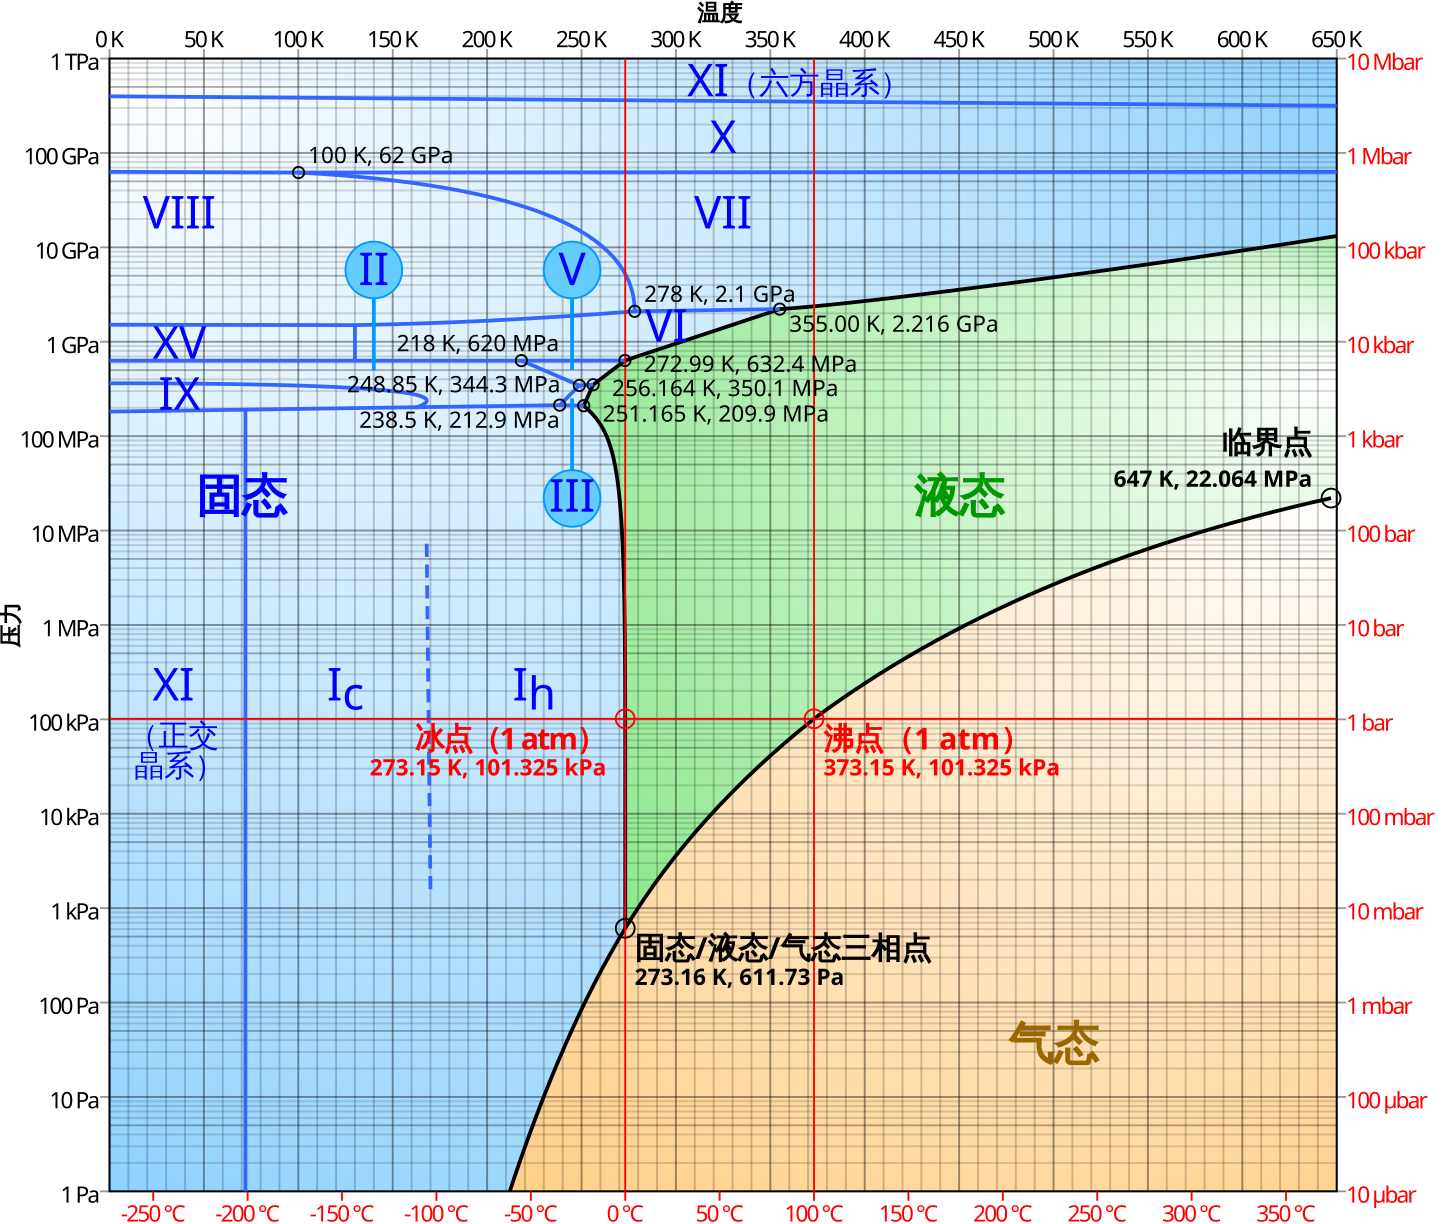
\includegraphics[scale=0.085]{./pictures/phase_diagram}
	\vspace*{0em}
	\subcaption{水的三相图}
	\end{minipage}
	\begin{minipage}{0.48\linewidth}
	\centering
	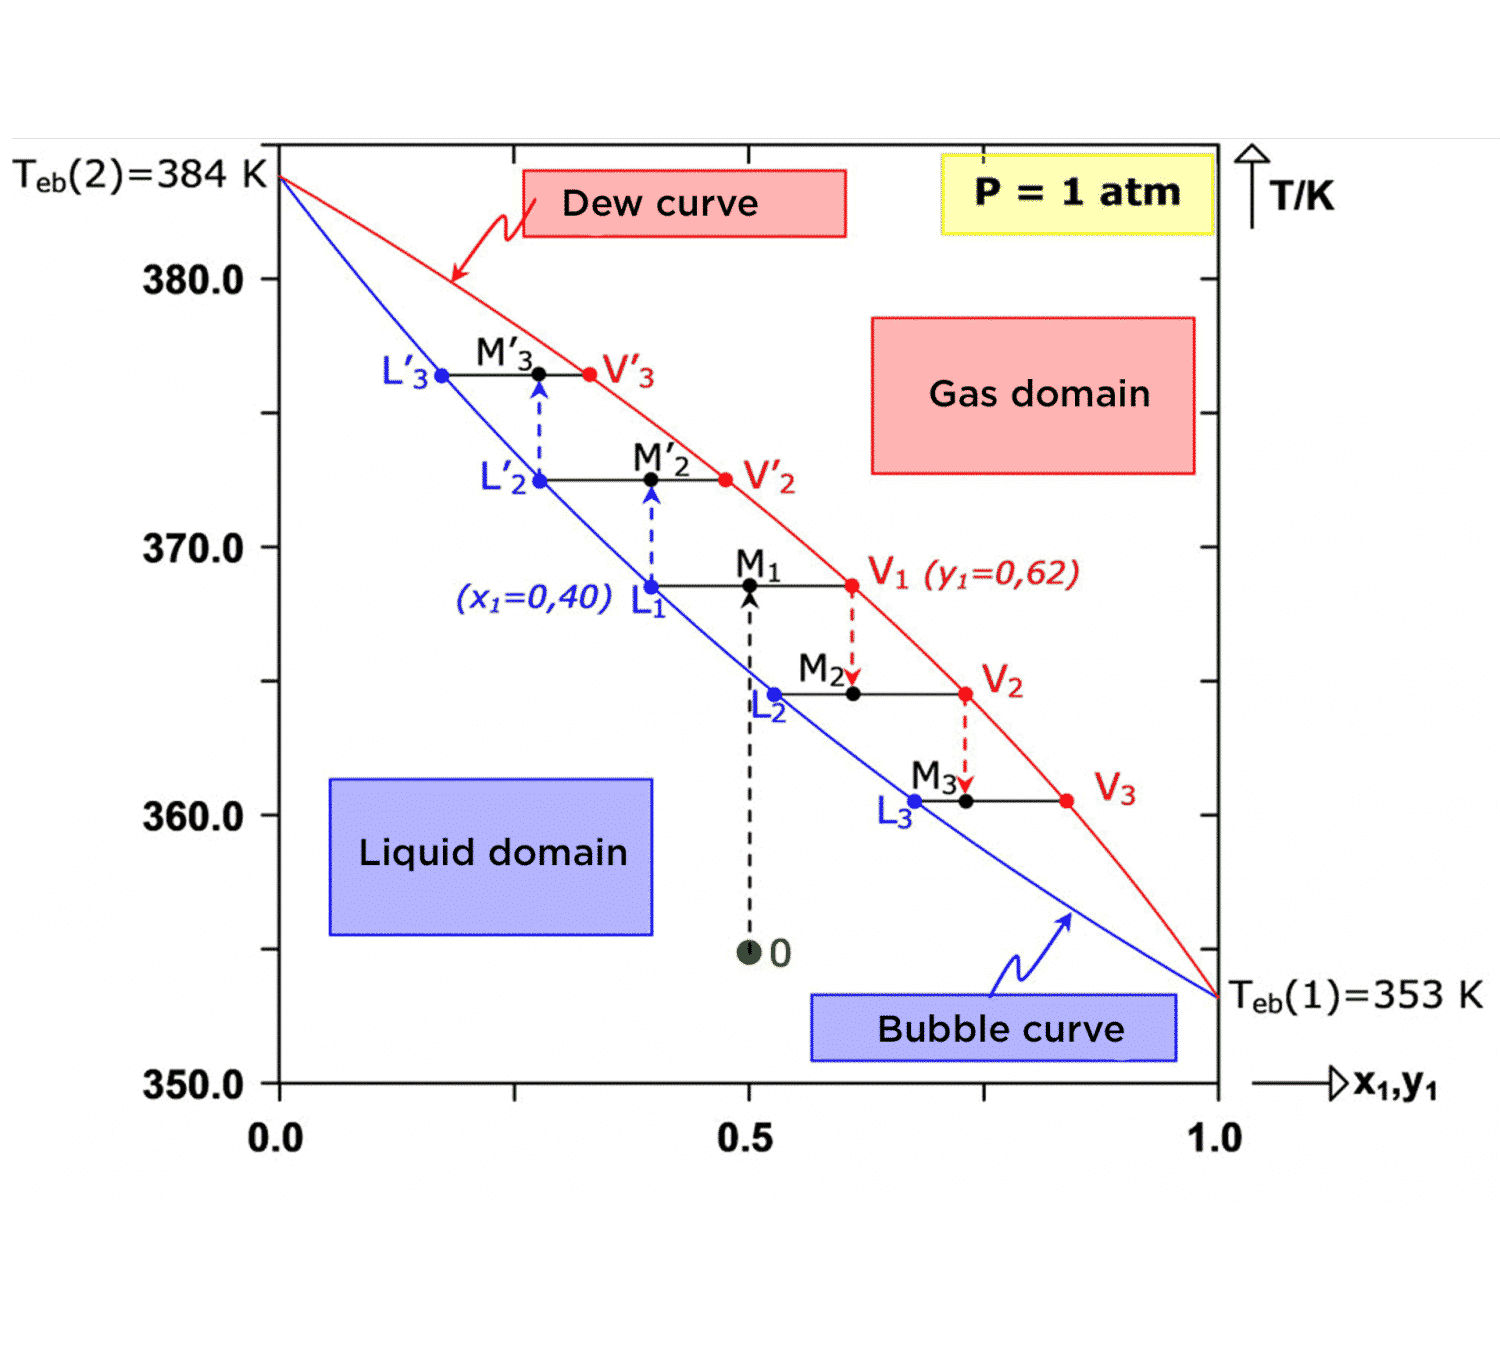
\includegraphics[scale=0.095]{./pictures/redistillation}
	\vspace*{-1.5em}
	\subcaption{苯——甲苯溶液于1 atm下的相图}
	\end{minipage}
	\caption{一些相图}
	\end{figure}

	\vspace*{-1em}

	\begin{itemize}
	
	\item 二组分理想液态混合物的相图的解析、杠杆规则、露点和泡点、恒沸物
	
	\item 生成化合物的二组分凝聚系统相图定性分析
	
	\end{itemize}
	
	\end{frame}
	
	\subsection{第七章}
	\begin{frame}
	
	{\color{blue}和之前(上册)几乎全部是经典热力学的内容不同,下册在其他体系中应用热力学原理之外,还有大量属于热力学的各成一节的系统性内容。因此,我会就每章各自可成体系介绍的内容进行总结归纳。}
	
	首先是第七章,其主要可分为三个部分:
	\begin{itemize}
	
	\item 电解质溶液的性质:包括了电解,电导,离子活度和离子强度
	
	\item 可逆电池的电动势及其应用

	\item 电极极化现象	
	
	\end{itemize}		
	
	第七章的主要原理:	
	\begin{itemize}
	
	\item Faraday定律:$Q=nzF$,Faraday常数$F=96485.340 \,{\rm C \cdot mol^{-1} }$
	
	\item 离子迁移数$t_\B$的概念和表达式
	\[
		t_\B = \frac{ Q_\B }{ Q_{\rm tot} }
	\]
	
	\item 电导$G$、电导率$\kappa$、电导池常数$K_{\rm cell}$的概念和定义
	\[
		K_{\rm cell} \equiv \kappa R
	\]
	
	\item 摩尔电导率$\Lambda_\m$的概念及定义
	\[
		\Lambda_\m(\B) \equiv \frac{ \kappa_\B }{ c_\B }
	\]
	
	\end{itemize}
	
	\end{frame}
	
	\begin{frame}
	
	\begin{itemize}
	
	\item Kohlrausch经验公式的适用范围
	\[
		\Lambda_\m(\B) = \Lambda^\infty_\m(\B) ( 1 - \beta \sqrt{c_\B} )
	\]
	
	\item  Kohlrausch离子独立运动定律
	\[
		\Lambda^\infty_\m = \nu_+ \Lambda^\infty_{\m,+} + \nu_- \Lambda^\infty_{\m,-}
	\]
	
	\item 弱电解质的解离度$\alpha$近似满足
	\[
		\alpha = \frac{ \Lambda_\m }{ \Lambda^\infty_\m }
	\]
	
	\item 离子平均活度$a_\pm$,离子平均活度系数$\gamma_\pm$和离子平均质量摩尔浓度$b_\pm$,电解质$\B$的活度$a_\B$之间的关系
	\begin{align*}
		a_\pm &\equiv ( a^{\nu_+}_+ a^{\nu_-}_- )^{\frac{1}{\nu}} = \gamma_\pm \frac{ b_\pm }{ b^{\,\ominus} } \\
		\gamma_\pm &= ( \gamma^{\nu_+}_+ \gamma^{\nu_-}_- )^{\frac{1}{\nu}} \\
		b_\pm &= ( b^{\nu_+}_+ b^{\nu_-}_- )^{\frac{1}{\nu}} \\
		a_\B &= a^\nu_\pm = a^{\nu_+}_+ a^{\nu_-}_- \\
		\nu &= \nu_+ + \nu_-
	\end{align*}
	
	\end{itemize}		
	
	\end{frame}
	
	\begin{frame}
	
	\begin{itemize}
	
	\item 电化学中的热力学量和电动势的关系
	\begin{align*}
		\Delta_\rr G_\m &= - z F E ,\\
		\Delta_\rr S_\m	&= - \left( \frac{ \partial \Delta_\rr G_\m }{ \partial T } \right)_p = z F \left( \frac{ \partial E }{ \partial T } \right)_p
	\end{align*}
	摩尔熵变$\Delta_\rr H_\m$和摩尔可逆恒压反应热$Q_{\rr,\m}$由
	\begin{align*}
		\Delta_\rr H_\m &= \Delta_\rr G_\m + T \Delta_\rr S_\m = -zFE + zFT \left( \frac{ \partial E }{ \partial T } \right)_p , \\
		Q_{\rr,\m} &= T \Delta_\rr S_\m = z F T \left( \frac{ \partial E }{ \partial T } \right)_p
	\end{align*}
	
	\item 若电池反应记为$\sum_\B \nu_\B \B=0$,则电池的Nernst方程为
	\[
		E = E^{\,\ominus} - \frac{ RT }{ zF }\ln{ \prod_\B a^{\nu_\B}_\B } = E_+ - E_-
	\]
	
	\item $E^{\,\ominus}$和$K^{\,\ominus}$的关系
	\[
		E^{\,\ominus} = \frac{ RT }{ zF } \ln{K^{\,\ominus}}
	\]
	
	\end{itemize}		
	
	\end{frame}
	
	\begin{frame}
	
	\begin{itemize}
	
	\item 电极反应的Nernst方程
	\[
		E_\pm = E^{\,\ominus}_\pm - \frac{ RT }{ zF } \ln{ \frac{ [a({\rm R})]^{ \nu_{\rm R} } }{ [a({\rm O})]^{ \nu_{\rm O} } }  }
	\]
	
	\item 原电池的书写规则和电解反应、电池反应的书写规则
	
	\item 分解电压、超电势和电极极化的概念,两类不同机理的电极极化
	\begin{align*}
		E_{\text{分解}} &= E_\rr + \Delta E_{\rm ir} + IR \\
		\Delta E_{\rm ir} &= \eta_{\text{阴极}} + \eta_{\text{阳极}}
	\end{align*}
		
	\end{itemize}		
	
	\end{frame}
	
	\begin{frame}
	
	本次课程课堂作业(基础):6.2,6.4,6.17,7.7
	
	\hspace*{\fill}	
	
	本次课程课后作业(可选):7.26
	
	\end{frame}		
	
	\section{第四部分}	
	
	\subsection{第十章}
	\begin{frame}
	
	第十章的主要原理:
	
	\begin{itemize}
	
	\item 比表面积$a_\s$、表面张力(表面功)$\gamma$的概念、物理意义和常见影响因素
	\[
		\gamma = \left( \frac{ \partial G }{ \partial A_\s } \right)_{T,p,n_\B}
	\]
	
	\item 弯曲液面的附加压力及其后果
		\begin{itemize}
	
		\item Laplace方程的适用前提和形式
		\[
			\Delta p = \frac{ 2\gamma }{ R }
		\]
		
		\item Kelvin公式的适用前提和形式
		\[
			RT \ln{ \frac{ p_\rr }{ p } } = \frac{ 2 \gamma M }{ \rho R }
		\]
		
		\item 亚稳态的行成和消除方法
	
		\end{itemize}
	
	\item 固体表面的吸附:单分子层吸附理论的假设和Langmuir吸附等温方程
	\[
		\theta \equiv \frac{ V^a }{ V^a_\m } = \frac{ bp }{ 1 + bp }
	\]
	
	\end{itemize}
	
	\end{frame}
	
	\begin{frame}
	
	\begin{itemize}
	
	\item 固——液界面的性质:接触角$\theta$和Young方程、润湿现象的分类
	\[
		\gamma^{\rm s} = \gamma^{\rm sl} + \gamma^{\rm l} \cos{ \theta }
	\]
	
	\item 液体表面的吸附:Gibbs吸附等温式给出了吸附量$\varGamma$
	\[
		\varGamma = - \frac{ a }{ RT } \frac{ \dif \gamma }{ \dif a } \approx - \frac{ c }{ RT } \frac{ \dif \gamma }{ \dif c } 
	\]	
	
	\item 表面活性剂的基本结构、分类和临界胶束浓度(CMC)
	
	\end{itemize}		
	
	\end{frame}
	
	\subsection{第十一章}
	\begin{frame}
	
	第十一章的主要原理:
	\begin{itemize}
	
	\item 反应速率的概念、和组分$\B$的变化速率的关系
		
	\item 基元反应、反应分子数的概念、质量作用定律、反应速率常数的概念
	
	\item 反应级数的概念、消耗(生成)速率常数和反应速率常数的关系
	
	\item 常见的级数反应的微分方程、半衰期计算方法
		\begin{itemize}
	
		\item 零级反应
		
		\item 一级反应
		
		\item 二级反应
	
		\end{itemize}
		
	\item 温度对反应速率的影响,Arrhenius方程和活化能$E_{\rm a}$的概念和物理意义
	\[
		\frac{ \dif \ln{k} }{ \dif T } = \frac{ E_{\rm a} }{ RT^2 }
	\]
	
	\item 活化能和摩尔恒容反应热$\Delta_\rr U^{\,\ominus}_\m$的关系
	\[
		E_{\rm a,1} - E_{\rm a,-1} = \Delta_\rr U^{\,\ominus}_\m
	\]
	
	\item 推导复合反应速率的近似方法
		\begin{enumerate}
		
		\item 选取控制步骤法
	
		\item 平衡态近似法
		
		\item 稳态近似法
	
		\end{enumerate}		
	
	
	\end{itemize}
	
	\end{frame}
	
	\subsection{第十二章}
	\begin{frame}
	
	第十二章的主要原理:	
	
	\begin{itemize}
	
	\item 胶体系统的概念,常见的三种胶体系统构成、性质和实例
	
	\item 胶体制备的常见制备方法(分散法和凝聚法)和净化方法(渗析法)
	
	\item 溶胶的光学性质
		\begin{itemize}
	
		\item Tyndall效应及其实质
	
		\item Rayleigh公式的前提和特点:$I \propto V^2$, $I \propto \lambda^{-4}$, $I \propto n^2-n^2_0 $,$I \propto C$
	
		\end{itemize}		
	
	\item 溶胶的动力学性质
		\begin{itemize}
		
		\item Brown运动的概念,Einstein-Brown平均位移公式
		\[
			\bar x = \sqrt{ \frac{ RTt }{ 3L\pi r \eta } }
		\]
		
		\item 球形粒子的扩散系数$D$的计算公式
		\[
			D = \frac{ RT }{ 6L\pi r \eta }
		\]
		
		\item Perrin分布律
		\[
			\ln{ \frac{ C_2 }{ C_1 } } = - \frac{ Mg }{ RT } \left( 1 - \frac{ \rho_0 }{ \rho } \right) ( h_2 - h_1 )
		\]
		
		\end{itemize}
	
	\end{itemize}
	
	\end{frame}
	
	\begin{frame}
	
	\begin{itemize}
	
	\item 溶胶的电学性质
		\begin{itemize}
	
		\item 四类电动现象
		
		\item 扩散双电层理论(Stern模型)
		
		\item 溶胶胶团结构的书写表达
	
		\end{itemize}
		
	\item 溶胶的稳定性的三个来源以及聚沉的方法
	
	\item 乳状液的分类、稳定性来源
	
	\item 高分子化合物溶液的渗透压计算,Donnan平衡
	
	\item 高分子化合物溶液的特性黏度$[\eta]$
	\[
		[ \eta ] = \lim_{\rho\rightarrow0} \left( \frac{ \eta_{\rm sp} }{ \rho }  \right)
	\]	
	和相对分子质量$M_\rr$的经验关系
	\[
		[ \eta ] = K M^\alpha_\rr
	\]
		
	
	\end{itemize}		
	
	\end{frame}
	
	\begin{frame}

	本次课程课堂作业(基础):10.3,11.10,11.44,12.12
	
	\hspace*{\fill}	
	
	本次课程课后作业(可选):10.5,10.9,10.16,12.2
	
	\hspace*{\fill}
	
	{\color{red}我非常感谢现在还在这里听我的讲述,坚持学习物理化学基础的同学们。祝你们未来学业精进,事业有成。}
	
	\end{frame}

\end{document}